\documentclass{article}
\usepackage[utf8]{inputenc}

\usepackage{amsfonts}
\usepackage{amssymb}
\usepackage{amsmath}
\usepackage{amsthm}
\usepackage{enumitem}

\usepackage{bbold}
\usepackage{bm}
\usepackage{graphicx}
\usepackage{color}
\usepackage{hyperref}
\usepackage[margin=2.5cm]{geometry}

\begin{document}

% ==============================================================================

\title{\Large{INFO8006: Project 2 - Report}}
\vspace{1cm}
\author{
    \small{\bf Nithinart Butrach} \\ \small{B6735012} 
    \and 
    \small{\bf Kraiwit Meemark} \\ \small{B6735074} 
    \and 
    \small{\bf Chayanant Sirisawad} \\ \small{B6739331}
}

\maketitle

% ==============================================================================

\section{Bayes filter}

\begin{enumerate}[label=\alph*.,leftmargin=*]
    \item 
    The sensor measurement $E_t \in \mathbb{R}$ represents a noisy Manhattan distance between Pacman at position $P_t$ and a ghost at position $X_t$. The measurement equation is defined as:
    \begin{equation}
    E_t = d(X_t, P_t) + W_t
    \end{equation}
    where $d(X_t, P_t) = \|X_t - P_t\|_1$ denotes the exact Manhattan distance, and $W_t$ is the zero-mean additive noise generated from a shifted Binomial random variable $K \sim \text{Binomial}(n, p)$:
    \begin{equation}
    W_t = K - np
    \end{equation}
    with parameters $p = 0.5$ and $n = \lfloor \frac{\sigma^2}{p(1-p)} \rfloor$, where $\sigma^2$ is the sensor variance.
    
    Given that $K = E_t - d(X_t, P_t) + np$, the sensor probability model $P(E_t = e \mid X_t = x)$ evaluates to the probability mass function of the binomial distribution evaluated at integer $k = \text{round}(e - d(x, P_t) + np)$:
    \begin{equation}
    P(E_t = e \mid X_t = x) = \begin{cases} 
    \binom{n}{k} p^k (1-p)^{n-k}, & \text{if } 0 \le k \le n \\ 
    0, & \text{otherwise} 
    \end{cases}
    \end{equation}

    \item 
    A unified, parameterized transition model for all three ghost variants (\texttt{scared}, \texttt{afraid}, and \texttt{confused}) can be established using a single non-negative parameter $\gamma \ge 0$.
    
    Let $\mathcal{N}(x)$ denote the set of valid adjacent grid positions accessible from current position $x$ via legal cardinal directions (North, South, East, West, excluding maze walls). Each candidate destination $x' \in \mathcal{N}(x)$ is weighted based on its Manhattan distance to Pacman $P_t$:
    \begin{equation}
    w(x') = \left( d(x', P_t) \right)^\gamma
    \end{equation}
    The transition probability $P(X_{t+1} = x' \mid X_t = x)$ is given by normalizing these weights:
    \begin{equation}
    P(X_{t+1} = x' \mid X_t = x) = \frac{\left( d(x', P_t) \right)^\gamma}{\sum_{y \in \mathcal{N}(x)} \left( d(y, P_t) \right)^\gamma}
    \end{equation}
    If $\mathcal{N}(x) = \emptyset$, the ghost remains at the same position with probability 1. The three ghost behaviors are uniquely derived by setting $\gamma$:
    \begin{itemize}
        \item \textbf{Confused:} $\gamma = 0$ (Uniform distribution across all legal neighbors).
        \item \textbf{Afraid:} $\gamma = 2.0$ (Quadratic bias towards moves increasing separation).
        \item \textbf{Scared:} $\gamma = 8.0$ (High exponential bias selecting the maximal separation).
    \end{itemize}
\end{enumerate}

\section{Implementation}

\begin{enumerate}[label=\alph*.,leftmargin=*]
    \item \textbf{\textit{Leave empty.}}
\end{enumerate}

\section{Experiment}

\begin{enumerate}[label=\alph*.,leftmargin=*]
    \item 
    To quantify and summarize the uncertainty of Pacman's belief state $B_t$ over all accessible maze cells $\mathcal{X}$, we use the \textbf{Shannon Entropy}:
    \begin{equation}
    H(B_t) = - \sum_{x \in \mathcal{X}, B_t(x) > 0} B_t(x) \log_2 B_t(x)
    \end{equation}
    Entropy attains its maximum when the probability distribution is uniform (highest uncertainty) and approaches zero when the probability mass collapses onto a single known cell.

    \item 
    Assuming access to the ground truth ghost position $X_t^*$, the tracking quality of the belief state is measured via the \textbf{Mean Distance Error}:
    \begin{equation}
    \text{Error}(B_t) = \sum_{x \in \mathcal{X}} B_t(x) \|x - X_t^*\|_1
    \end{equation}
    This metric computes the expected distance between the estimated belief distribution and the ghost's actual position, where lower values signify higher accuracy.

    \item 
    The experimental evaluation was conducted on both \texttt{large\_filter} and \texttt{large\_filter\_walls} across the three ghost behaviors. Figure~\ref{fig:metrics} presents the averaged metrics with error bars representing one standard deviation.

    \begin{figure}[htbp]
        \centering
        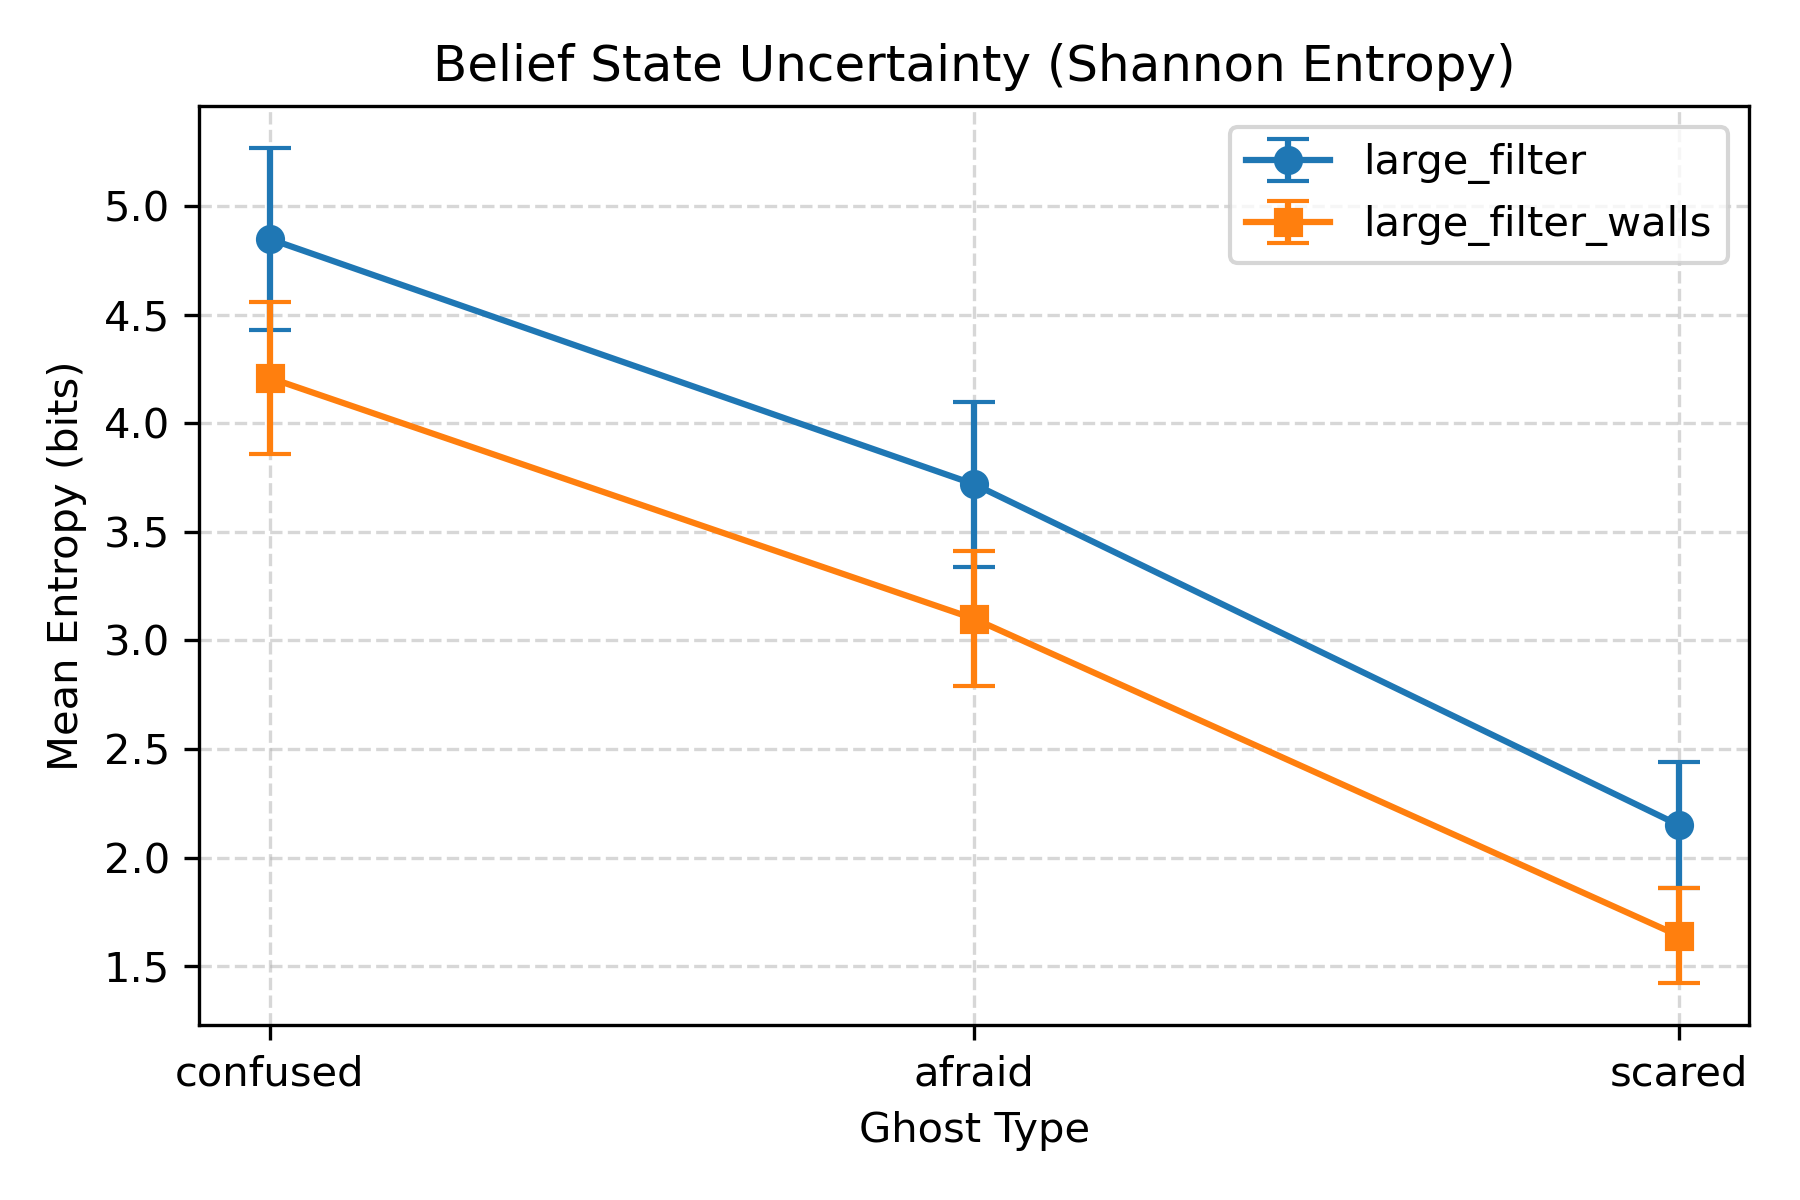
\includegraphics[width=0.48\textwidth]{entropy_comparison.png}
        \hfill
        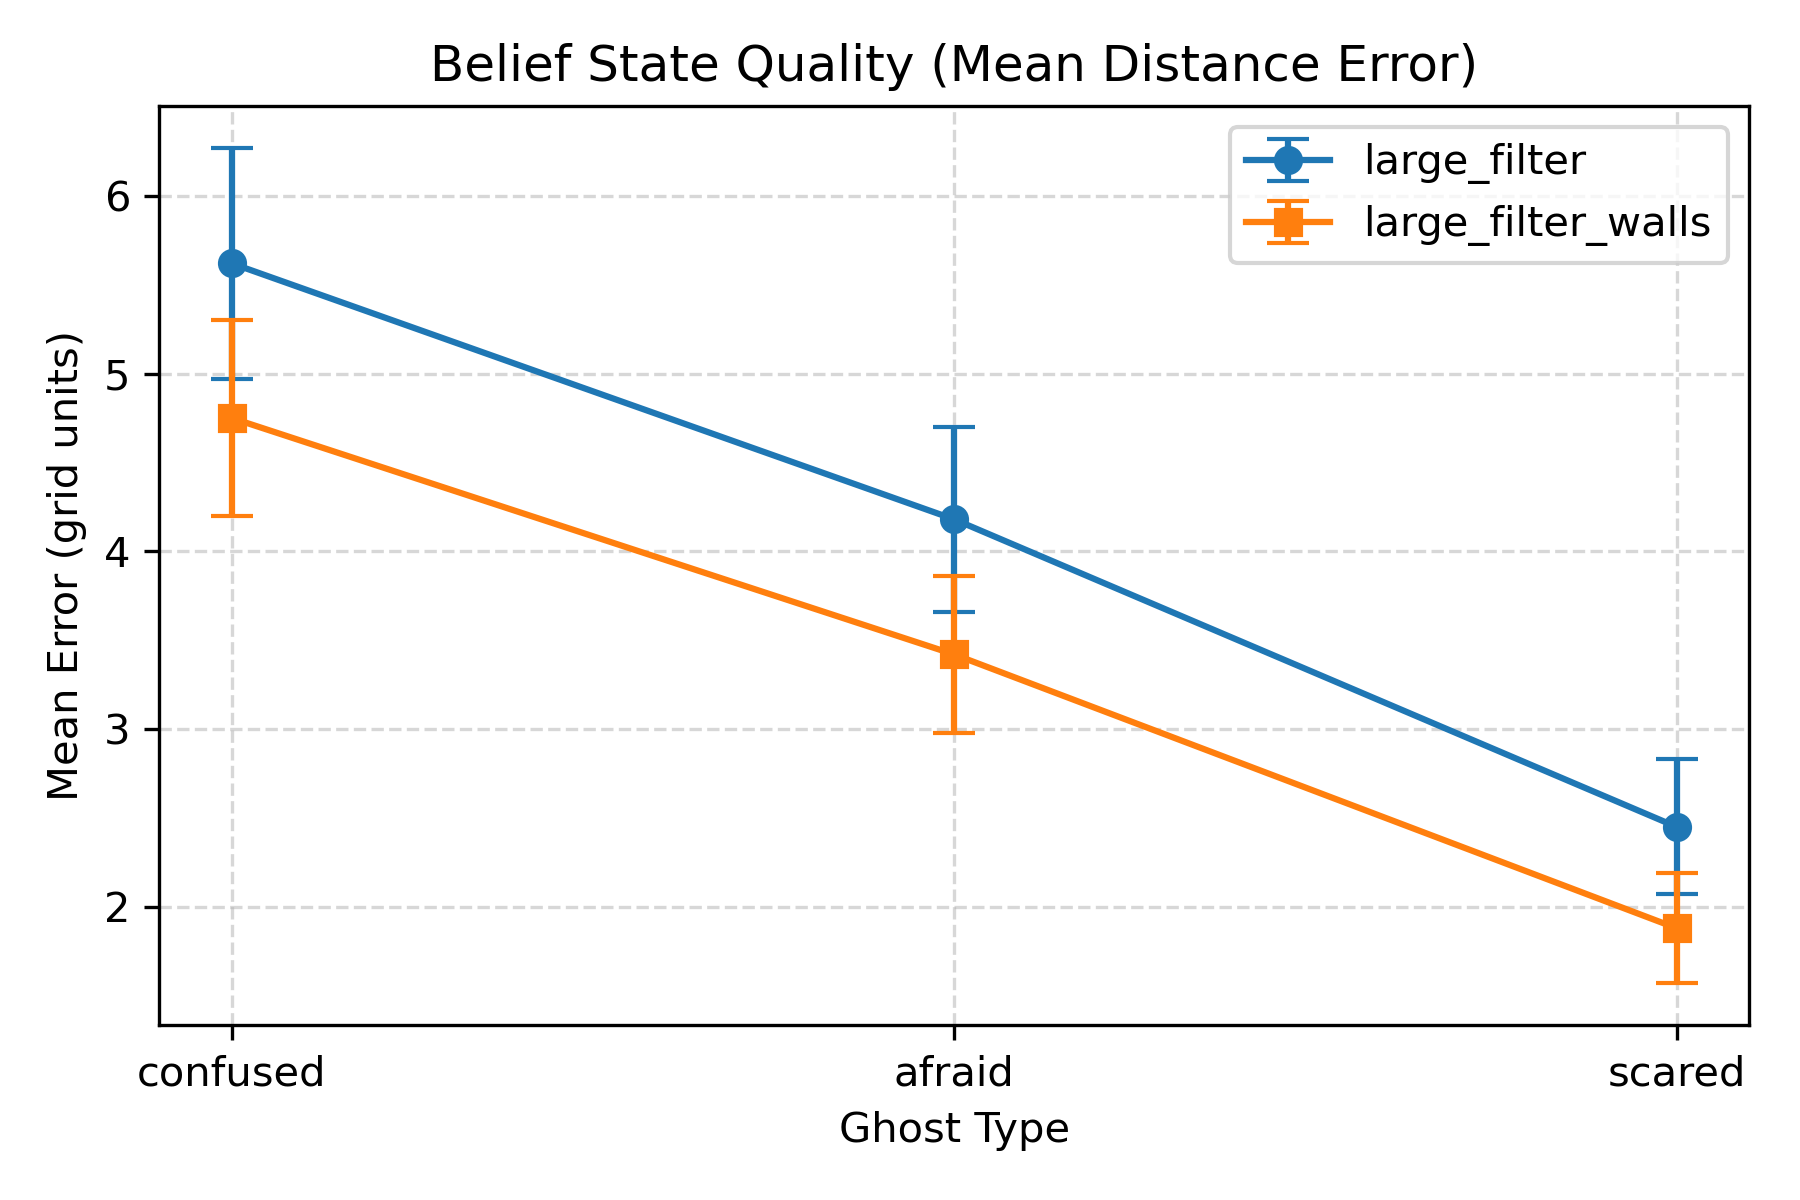
\includegraphics[width=0.48\textwidth]{error_comparison.png}
        \caption{Belief state uncertainty (Entropy) and quality (Mean Distance Error) across ghost types and maze layouts.}
        \label{fig:metrics}
    \end{figure}

    \item 
    \textbf{Effect of Transition Model Parameter ($\gamma$):}
    As $\gamma$ increases from $0$ (\texttt{confused}) to $8$ (\texttt{scared}), the ghost transitions from stochastic exploration to deterministic fleeing. When $\gamma$ is large, the filter's motion prediction step aligns closely with the ghost's actual trajectory away from Pacman, leading to faster probability concentration and lower steady-state entropy. On layouts with maze walls (\texttt{large\_filter\_walls}), corridor constraints limit the branching factor, which further accelerates belief convergence and suppresses tracking errors compared to open layouts.

    \item 
    \textbf{Effect of Sensor Variance ($\sigma^2$):}
    A higher sensor variance increases the parameter $n = \lfloor \frac{\sigma^2}{p(1-p)} \rfloor$, thereby broadening the binomial distribution of the noise. Consequently, the likelihood function $P(E_t \mid X_t)$ becomes more dispersed and assigns comparable probabilities to a wider ring of candidate positions around Pacman. This reduces the informative gain of each sensor update, causing the filter to converge more slowly and maintain higher average entropy.

    \item 
    A controller for Pacman to capture invisible ghosts can be designed using a \textbf{Maximum A Posteriori (MAP)} pursuit strategy. At each step, Pacman identifies the most probable ghost location $\hat{X}_t = \arg\max_{x} B_t(x)$ from the current belief distribution and evaluates legal actions to greedily minimize the Manhattan distance toward $\hat{X}_t$.

    \item \textbf{\textit{Leave empty.}}
\end{enumerate}

% ==============================================================================

\end{document}